\lstset{language=JavaScript}

\block{
	\section{Web frontend}

	\subsection{\mt{Áttekintés}{}}

	\p{\mt{%
		A webes frontend html része több fájlba van tagolva az olvashatóság érdekében.
		A html nagy része sablon amit a javascript használ az oldal megjelenítéséhez.
		Ez lehetővé teszi az újratöltés mentes navigálást.
	}{}}
}

\block{
	\subsection{Építés}
	
	\p{\mt{%
		A frontend építéséhez a Linux alapú rendszeren \code{build} vagy Windowson \code{build.bat} fájlt kell futtatni.
		Ez kétrehozza az \code{index.html} fájlt a széttagolt html fájlokból.
	}{}}
}

\block{
	\subsection{\mt{Template osztály}{}}
	
	\p{\mt{%
			A \code{Template} osztály segíti a html minták kezelését.
			A htmlben osztályokkal vannak megjelölve azok az elemek amiket JavaScript kód módosít.
			A \code{get} funkció ezek az elemek lekérését segíti.
			A \code{getNode} funkció visszaadja az új template gyökér elemét.
		}{}
		
		\lstinputlisting{generated/web.template.js}
	}
}

\begin{landscape}
	\begin{figure}
		\centering
		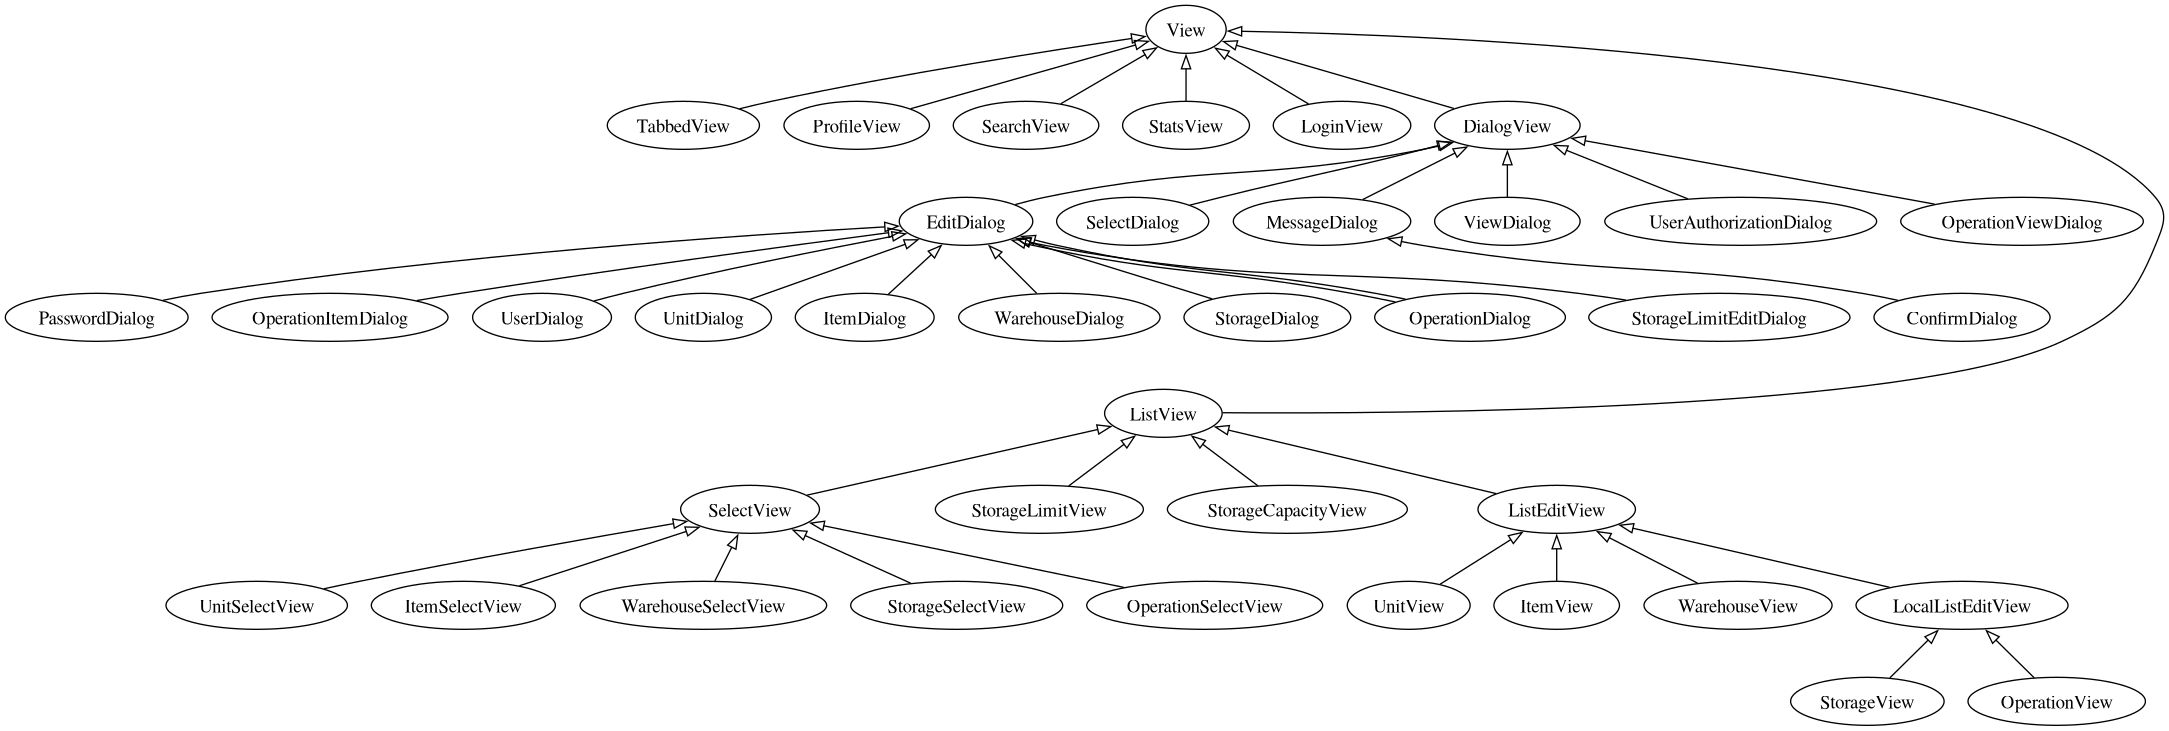
\includegraphics[width=\linewidth]{webfrontend.classes.png}
		\caption{\mt{Osztálydiagramm}{}}
	\end{figure}
\end{landscape}

\block{
	\subsection{\mt{View osztály}{}}
	
	\p{\mt{%
			A \code{View} osztály a felhasználói felület részek szülőosztálya.
			Ebben az osztályban az \code{initTemplate} metódus egyszer hívódik meg és a feladata az, hogy inicializálja a felhasználói felület részt.
		}{}
		
		\lstinputlisting{generated/web.view.js}
	}
}

\block{
	\subsection{\mt{ListView osztály}{}}
	
	\p{\mt{%
			A \code{ListView} osztály a listák szülőosztálya. Ebben a listában lehet
			lapozni, keresni és újratölteni. A \code{load} funkció feladata, hogy a megadott
			paraméterekre (keresési szöveg, archivált-e, kezdő pozíció és mennyiség)
			vissza adjon egy \code{Promise} objektumot, amely később vissza adja majd a betöltött értékeket.
			A töltés animáció egész addig látható a felületen, amíg a Promise
			nem ad vissza értéket vagy hibát. A \code{createItemCard} funkció feladata,
			hogy a betöltött értékeket vizualizálja.
		}{}
		
		\lstinputlisting{generated/web.listview.js}
	}
}

\block{
	\subsection{\mt{ListEditView osztály}{}}
	
	\p{\mt{%
			A \code{ListEditView} osztály a \code{ListView} osztályt szerkesztési menüvel egészíti ki.
			A \code{createEditView} funkció feladata az, hogy létre hozza a szerkesztési menüt.
			A \code{item} a szerkeszteni kívánt érték. Ez \code{null} ha újat akarunk létrehozni.
			Az \code{item\_callback} funkciót kell meghívnia a menünek a mentéshez.
			Ennek a paraméterei az eredeti érték és az új érték.
			A \code{save} funkció feladata az új vagy módosított érték mentése.
		}{}
		
		\lstinputlisting{generated/web.listeditview.js}
	}
}

\block{
	\subsection{\mt{SelectView osztály}{}}
	
	\p{\mt{%
			A \code{SelectView} osztály a kiválasztási listák szülőosztálya.
			Ez az osztály a \code{ListView} osztályt egészíti ki és ezért ebben a listában is lehet lapozni, keresni és újratölteni.
		}{}
		
		\lstinputlisting{generated/web.selectview.js}
	}
}

\block{
	\subsection{\mt{DialogView osztály}{}}
	
	\p{\mt{%
			A \code{DialogView} osztály a felugró menük szülőosztálya. A \code{hasOk} funkció
			igazat ad, amennyiben ennek a menünek van OK gombja. Ebben az esetben implementálni kell az \code{ok} funkciót.
			Ez a funkció az OK gomb lenyomásakor hívódik meg és egy \code{Promise} objektumot ad vissza, majd a töltés animáció
			egész addig látható lesz, amíg ez az objektum kész nem lesz.
		}{}
		
		\lstinputlisting{generated/web.dialogview.js}
	}
}

\block{
	\subsection{\mt{EditDialog osztály}{}}
	
	\p{\mt{%
			A \code{EditDialog} osztály a szerkesztési menük szülőosztálya.
			A \code{getItem} funkció visszaadja a módosított értéket vagy hibát ha rosszul van kitöltve a menü.
		}{}
		
		\lstinputlisting{generated/web.editdialog.js}
	}
}



